\documentclass{SBCbookchapter}
\usepackage[utf8]{inputenc}
\usepackage[T1]{fontenc}
\usepackage[english]{babel}
\usepackage{graphicx,caption}
\usepackage{physics}
\usepackage{amsmath}
\usepackage{float}
\usepackage{lscape}
\usepackage{multicol}
\usepackage{wrapfig}
\usepackage{adjustbox}

\graphicspath{{Figures/}}
\author{Prajeesh A Gopinathan}
\title{Spectral Transforms}

\begin{document}
\maketitle

In a spectral global model one part of the computations are made in spectral space (horizontal derivatives, semi-implicit time stepping, horizontal diffusion), and the other part in grid-point space on a grid defined by a Gaussian quadrature. It is therefore necessary to perform spectral transforms from spectral space to gird-point space and vice-versa. The present chapter aims at giving the details of the spectral method used in IITM's Atmospheric Model.

\section{Spectral Representation}
The spectral representation of a state variable $A$ on a given vertical layer above the surface of a sphere is definded by an approximation to the variable by truncated series of spherical harmonics using a triangular truncation at wavenumber N, given as:
\begin{equation}
A(\lambda,\mu) = \sum_{m=0}^N \sum_{n=|m|}^{N} A_{n}^{m} P_{n}^{m} (\mu) e^{im\lambda}
\end{equation}
 where $\mu=sin\theta$, $\theta$ is latitude, $\lambda$ is longitude, and $P_{n}^{m}(\mu)$ is the associated Legendre function, $m$ is the fourier wave number.
Transforming from grid-point space to spectral space involves performing an fourier transform for each line of constant latitude, 
\begin{equation}
A_{m}(\mu) = \frac{1}{2\pi} \int_{0}^{2\pi} A(\lambda,\mu) e^{-im\lambda} d\lambda
\end{equation}

followed by a integral over latitudes using a Gaussian quadrature to obtain the spherical harmonics,

\begin{equation}
A_{n}^{m} = \sum_{j=1}^{J} A^{m}(\mu_j)P_{n}^{m}(\mu_j) \omega_j
\end{equation}
where, $A^m$ is the mth Fourier coefficient, $\omega_j$ is the Gaussian quadrature weight corresponding to Gaussian latitude $\mu_j$ and $J$ total number of latitudes. The operation count this integral can be halved by making use of the symmetry properties of the Legendre polynomials about the equator:

\begin{equation}
\left.
\begin{array}{ll}
P_n^m(-\mu) = P_n^m(\mu)\\
H_n^m(-\mu) = -H_n^m(\mu)
\end{array}
\right\} \text{for n-|m| even, and}
\left.
\begin{array}{ll}
P_n^m(-\mu) = -P_n^m(\mu)\\
H_n^m(-\mu) = H_n^m(\mu)
\end{array} 
\right\} \text{for n-|m| odd}
\label{eqn_sym}
\end{equation}
The fourier transforms are performed numerically by using Fast Fourier Transfroms.

\section{Horizontal Derivatives}
\subsection{Meridional derivative relative to latitude $\theta$ }
For a variable A, meridional derivative can be derived from from spectral space using two methods. First method is using the formula:
\begin{equation}
\left(\cos\theta\pdv{A}{\theta}\right)_{n}^m = -(n-1)e_{n}^m A_{n-1}^m + 
(n+2)e_{n+1}^m A_{n+1}^m
\end{equation}
where, $e_0^0=0$ and $e_n^m = \sqrt{\frac{n^2-m^2}{4n^2-1}}$. And second method is using formula for transformation from spectral to grid point space:
\begin{equation}
\cos\theta\pdv{A}{\theta} = \sum_{m=0}^{N} \sum_{n=|m|}^{N} A_{n}^{m} H_{n}^{m} (\mu) e^{im\lambda}
\end{equation}
where, $H_n^m(\mu) = -ne_{n+1}^m P_{n+1}^m(\mu) + (n+1)e_n^m P_{n-1}^m(\mu)$.

\subsection{Zonal derivative relative to longitude $\lambda$}
For a variable A , zonal derivative is discretized in spectral space by the
following formula:
\begin{equation}
\left(\pdv{A}{\lambda}\right)_n^m = imA_n^m
\end{equation}
This can also be derived from multiplication of $im$ on fourier coefficients.

\section{Relationship between dimension in spectral space and grid point space}
Spectral space is defined by a triangular truncation $N$. Grid point space has $NLAT$ latitudes and maximum number of longitudes equal to $MAXLON$. $NLAT$ and $MAXLON$ are always even integers, where $MAXLON=20+(NLAT/2-1)*4$.

For a quadratic Gaussian grid, the relationship between spectral space and grid point space to avoid aliasing on quadratic terms is given by $N \leq (2*NLAT-1)/3$.
In a semi-Lagrangian scheme as the advective quadratic terms disappear, it is possible to use a linear Gaussian grid, which has a relation $N \leq NLAT-1$.
For a cubic Gaussian grid, the relationship is $N \leq NLAT/2 -1 $

\section{Octahedral reduced Gaussian grid}
To save memory and computation time (in particular in the physical parameterizations) and to maintain a quasi-isotropic grid the number of longitudes per latitude circle is reduced as we move towards the poles from equator. 
The method used to reduce the number of grid points towards pole is inspired by a regular triangular mapping onto an octahedron, which corresponds to a reduction of 4 points per latitude circle, one per face of the octahedron \cite{malardel_new_2016}. The resulting grid is called the "octahedral reduced gaussian grid". A octahedral reduced Gaussian grid can be generated using the formula: $NLON_j = NLON_{pole} + 4*(jj-1)$, where $jj=j$, if $j \leq NLAT/2$, else $jj=NLAT-j+1$, $j$ is latitude index, $NLON_{pole}$ is the number of grid points at first latitude near to pole, $NLON_j$ is the number of grid points at $j$th latitude. In general, $NLON_{pole}$ is taken as 20. Figure \ref{fig1} gives an example of octahedral reduced grid.

\begin{figure}[H]
	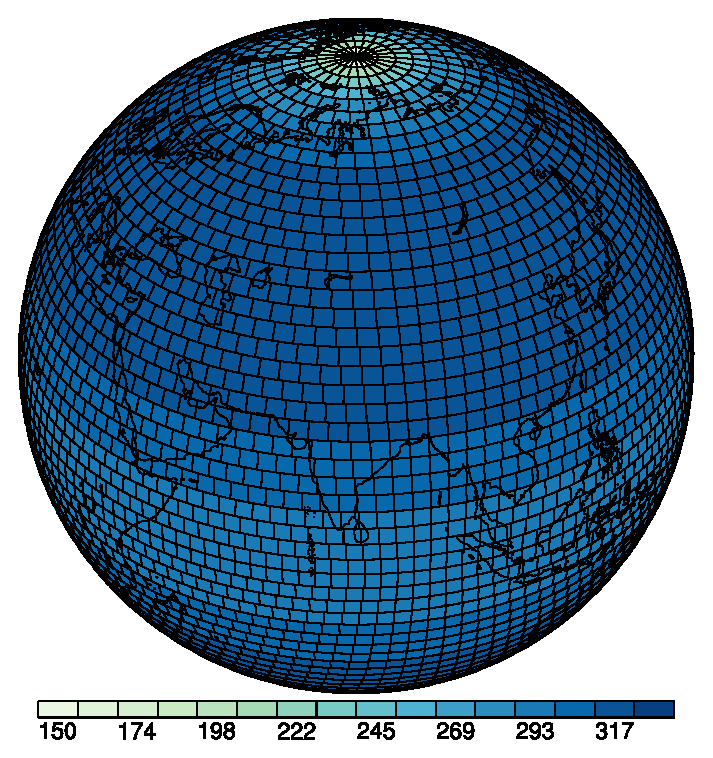
\includegraphics[width=\linewidth]{red_sphere.eps}
	\caption{A schematic representation of octahedral reduced grid having 64 latitude circles ($NLAT=64$). The color shading is grid resolution in kilometers.}
	\label{fig1}
\end{figure}

\section{Packed-grid}
A 2-dimensional domain decomposition of reduced Gaussian grid without any special rearrangement will lead to a large load imbalance between the processors. This is shown in figure~\ref{fig2}, the gray points in the figure shows the invalid points which are unevenly distributed between the processors. It can be seen from the figure that such decomposition would lead to very few number of valid points in some processors and large number in others. To overcome this issue the reduced Gaussian grid points are re-arranged in a way to ensure a even distribution of grid points when doing a domain decomposition and this new grid is called as Packed-grid (or P-grid). Figure~\ref{fig3} shows the corresponding packed-grid of the reduced Gaussian grid shown in figure~\ref{fig2}.
A packed-grid is generated by following steps:  
\begin{itemize}
	\item Assume that the indexing of the latitude circle is follows: $S_1$ to $S_{n}$ for the latitudes in southern hemisphere starting from pole to equator and $N_1$ to $N_{n}$ for northern hemisphere, $n=NLAT/2$, where $NLAT$ is total number of latitudes.
	\item Then, $i^{th}$ row of P-grid for southern hemisphere ($PS_{i}$) is formed by joining $S_{i}$ and $S_{n-i+1}$, where $i$ is from $1$ to $n/2$, similarly for northern hemisphere P-grid ($PN_{i}$).
	\item The final P-grid is formed by shuffling the rows of P-grid of southern hemisphere and northern hemisphere. i.e, $P_1$ will be $PS_1$, $P_2$ will be $PN_1$, $P_3$ will be $PS_2$, $P_4$ will be $PN_2$, so on and so forth.
\end{itemize}

\begin{figure}[H]
	\centering
	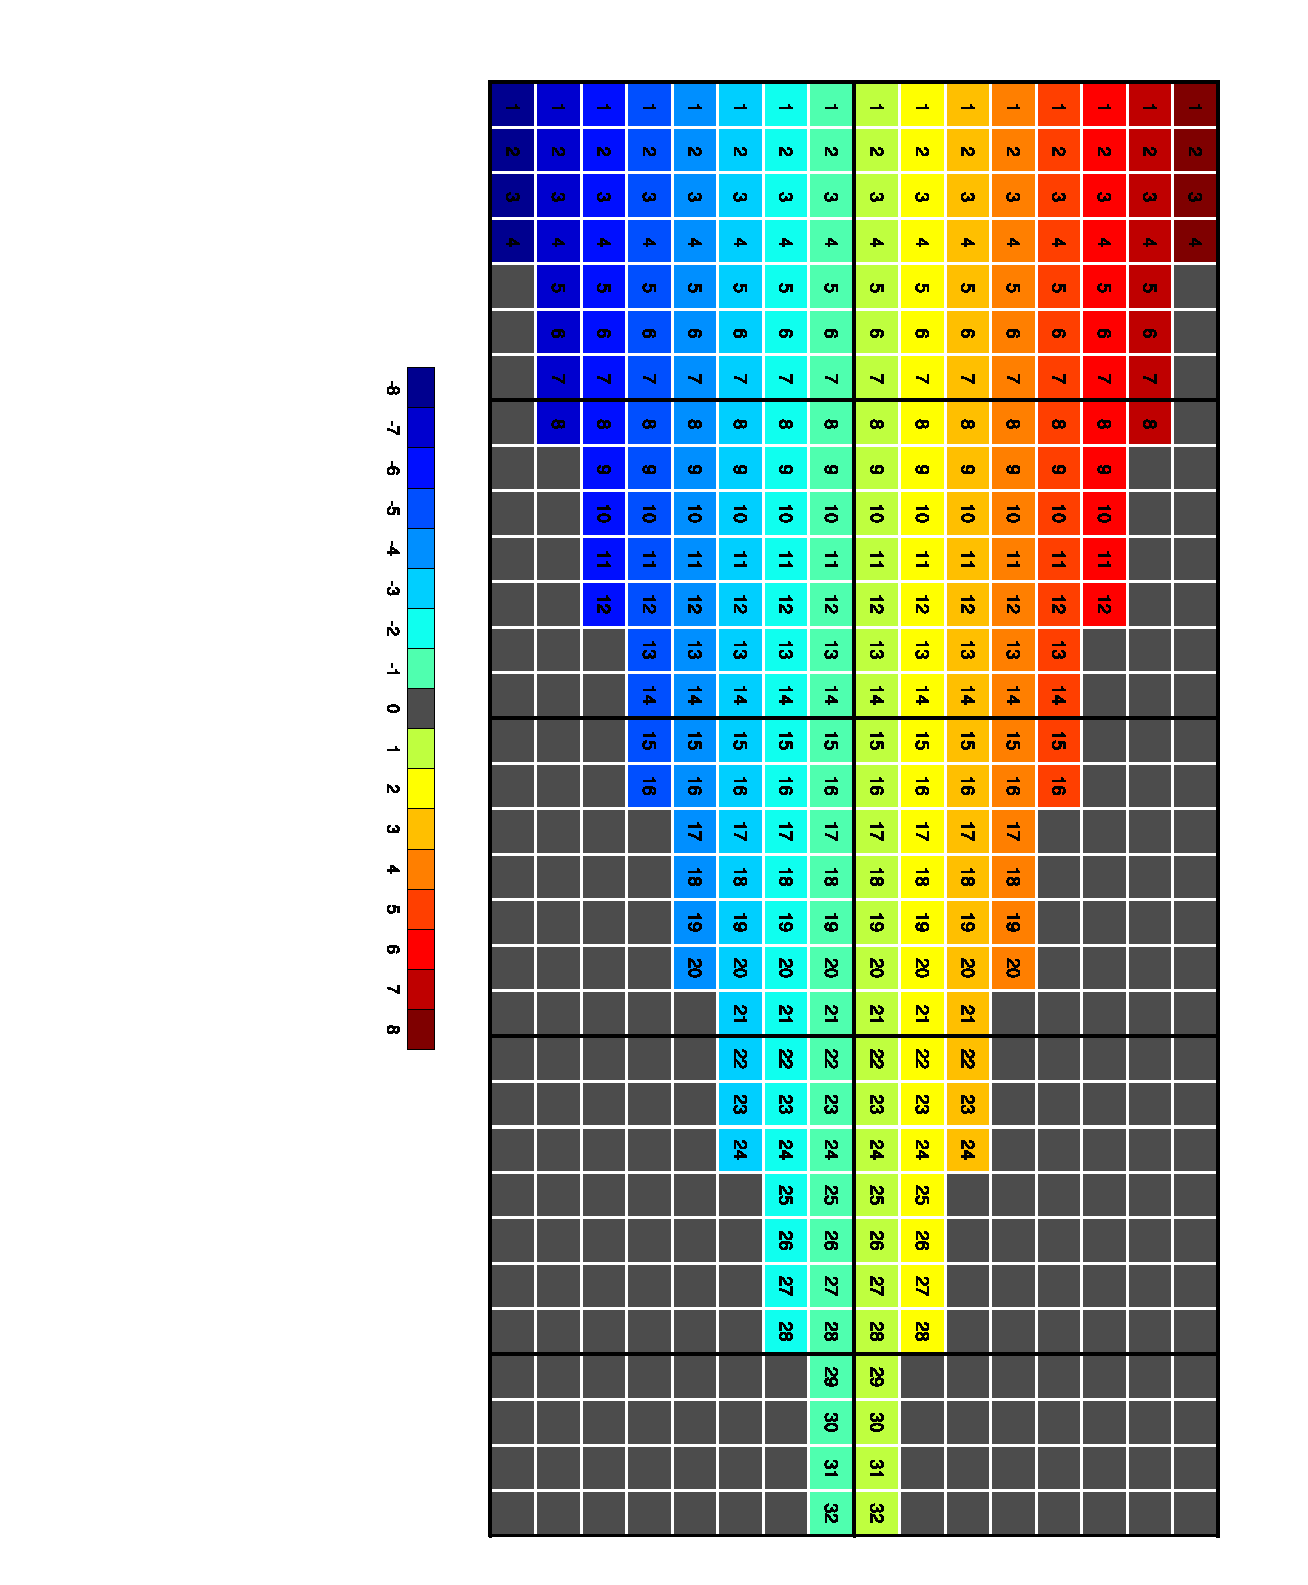
\includegraphics[angle=90,width=0.9\textwidth]{grid3.eps}
	\caption{A schematic representation of octahedral reduced grid having 16 latitude circles ($NLAT=16$) as a 2 dimensionally decomposed computer array. The color shading is the latitude indexing starting from -8 to 8, where the negative values represent southern hemisphere and positive values are northern hemisphere. The colored small square is a single grid point and the numbering inside the box is longitudinal index, and the gray squares are invalid elements. Black lines represents the domain decomposition, all the grid points enclosed by the black line is in one processor.}
	\label{fig2}
\end{figure}

\begin{figure}[H]
	 \begin{adjustbox}{addcode={\begin{minipage}{\width}}{\caption{%
						Here is a caption of the figure which is so long that 
						it has to be wrapped over multiple lines, but should 
						not exceed the width (height after the rotation) of the image.
			}\end{minipage}},rotate=90,center}
	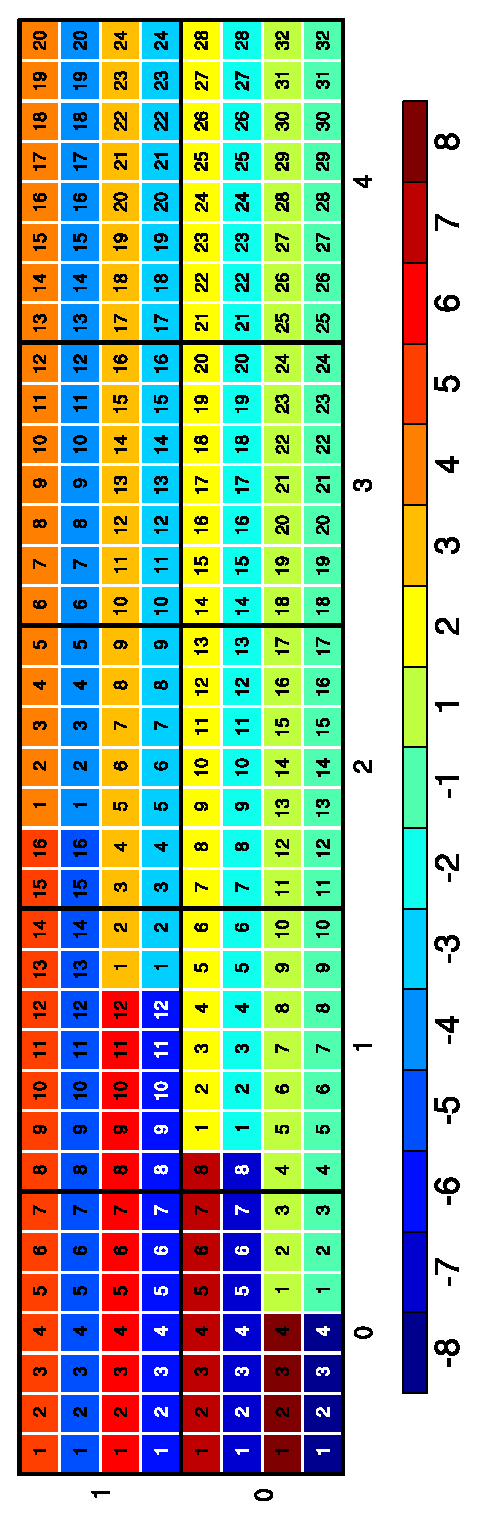
\includegraphics[angle=270]{P-grid_dom.eps}
\end{adjustbox}
	\label{fig3}
\end{figure}

\begin{wrapfigure}{r}{0.4\textwidth}
	\centering
	\captionsetup{width=.4\textwidth}
	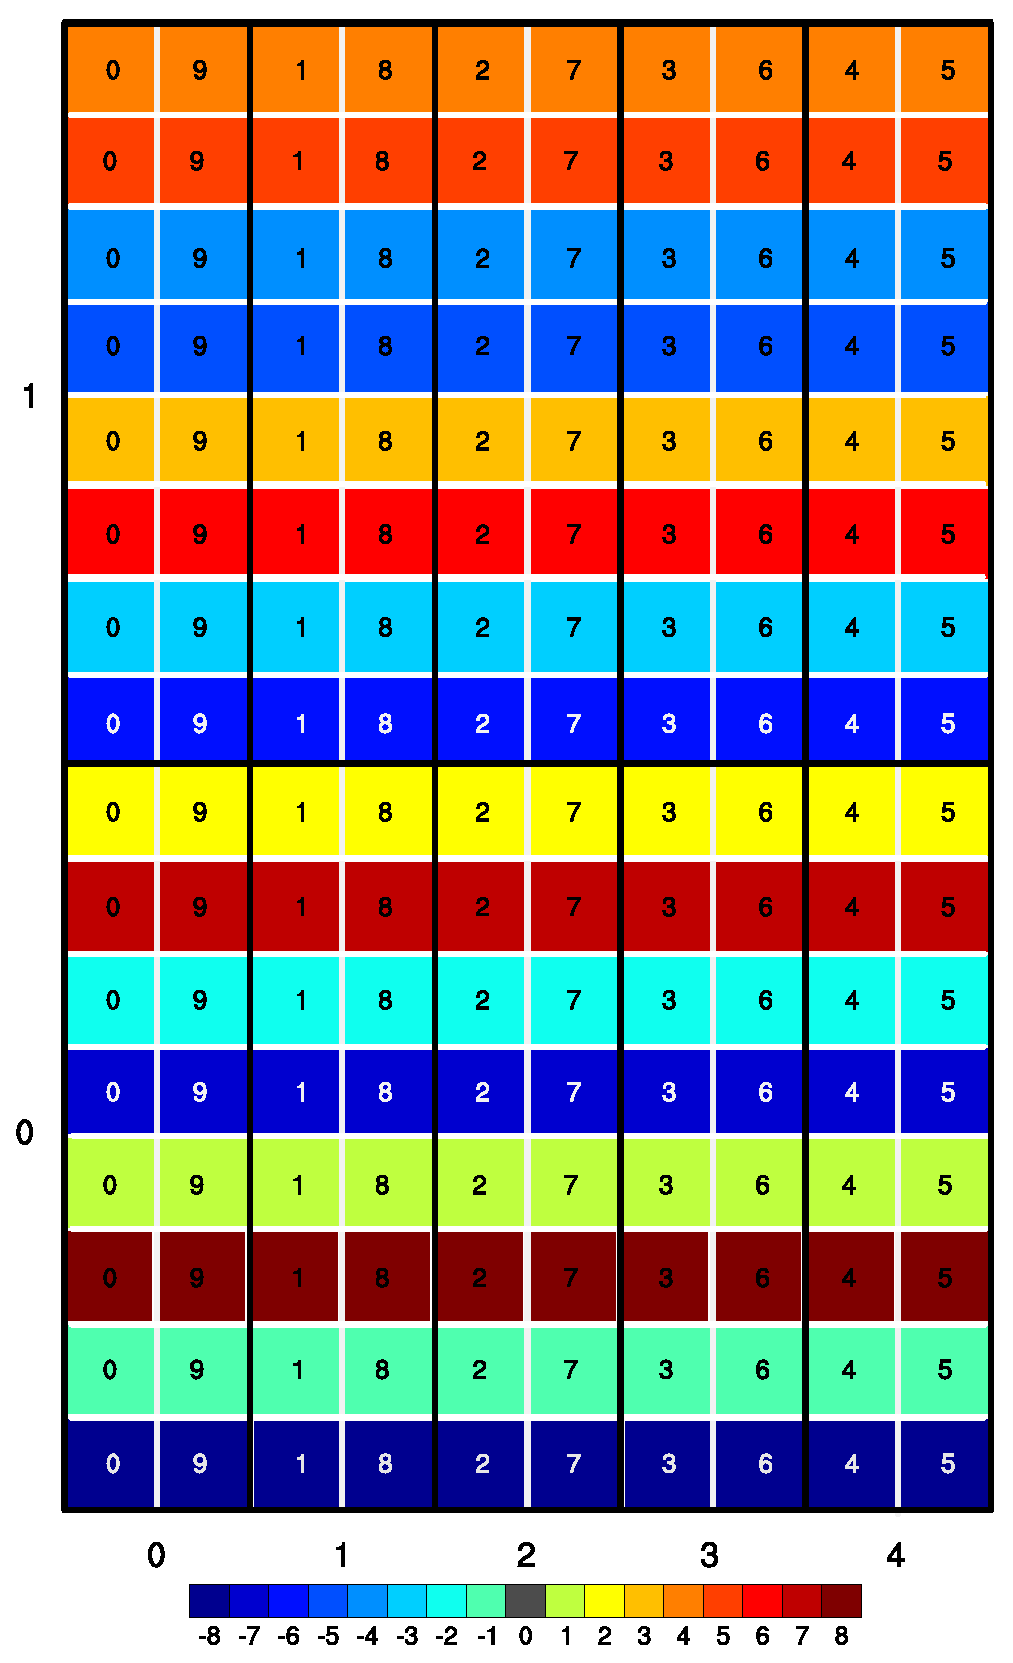
\includegraphics[width=0.45\textwidth]{fourier_dom.eps}
	\caption{Same as figure~\ref{fig2}, except that the grid has been re-arranged to form a Packed-grid.}
	\label{fig4}
\end{wrapfigure}

The last step of hemispheric shuffling is done to ensure that the corresponding symmetric latitude circles from the two hemispheres are next to each other and are in the same processors when having a domain decomposition in the y-direction, by which the operations described in  equation~\ref{eqn_sym} can be done locally within a processor without any communication.



\bibliographystyle{unsrt}
\bibliography{reference.bib}

\end{document}